\documentclass[a4paper,11pt]{article}
\usepackage[T1]{fontenc}
\usepackage[utf8]{inputenc}
\usepackage{lmodern}
\usepackage{microtype}
\usepackage[top=2.5cm,bottom=2.5cm,left=2.5cm,right=2.5cm]{geometry}
\usepackage{booktabs}
\usepackage{graphicx}
\usepackage{xcolor}
\usepackage{array}
\usepackage[colorlinks=true,urlcolor=blue,linkcolor=blue]{hyperref}
\usepackage{fancyhdr}
\usepackage{amssymb}
\usepackage{pdflscape}

\definecolor{accent}{RGB}{52,152,219}

\pagestyle{fancy}\fancyhf{}
\lhead{\small\itshape Effect of cocoa flavanol supplementation for the prevention }
\rhead{\small\itshape Flavonoid research --- Paper Report}
\rfoot{\small\thepage}
\renewcommand{\headrulewidth}{0.4pt}

\begin{document}

\begin{center}
  {\LARGE\bfseries Effect of cocoa flavanol supplementation for the prevention of cardiovascular disease events: the COcoa Supplement and Multivitamin Outcomes Study (COSMOS) randomized clinical trial}\\[0.4em]
  {\large\color{accent} Flavonoid research}\\[0.25em]
  {\normalsize 2022.0 \quad American Journal of Clinical Nutrition}\\[0.15em]
  {\small Study type: RCT}\\[0.1em]
  {\small\url{https://doi.org/10.1093/ajcn/nqac055}}
\end{center}
\vspace{0.4em}\noindent\rule{\linewidth}{0.5pt}\vspace{0.4em}



\section*{Citation Metrics}

\begin{tabular}{lr}
\toprule
Metric & Value \\
\midrule
    Total citations & 172 \\
    Citing papers in Flavonoid research corpus & 51 \\
    References in Flavonoid research corpus & 33 \\
    Authors & 13 \\
    Open access & No \\
\bottomrule
\end{tabular}

\section*{Top Citing Papers (Flavonoid research corpus)}

\begin{tabular}{p{1cm}p{8.5cm}p{3.5cm}r}
\toprule
Year & Title & Journal & Citations \\
\midrule
    2022.0 & Micronutrient Supplementation to Reduce Cardiovascular Risk & Journal of the American College of  & 185 \\
    2022.0 & Flavan-3-ols and Cardiometabolic Health: First Ever Dietary Bioac & Advances in Nutrition & 101 \\
    2022.0 & From Cocoa to Chocolate: Effect of Processing on Flavanols and Me & International Journal of Molecular  & 81 \\
    2022.0 & Effects of cocoa extract and a multivitamin on cognitive function & Alzheimer s \textbackslash{}& Dementia & 79 \\
    2022.0 & Revisiting the bioavailability of flavan-3-ols in humans: A syste & Molecular Aspects of Medicine & 63 \\
    2023.0 & Dietary flavanols restore hippocampal-dependent memory in older a & Proceedings of the National Academy & 50 \\
    2024.0 & Effect of multivitamin-mineral supplementation versus placebo on  & American Journal of Clinical Nutrit & 35 \\
    2024.0 & Potential of dietary polyphenols for protection from age-related  & Nutritional Neuroscience & 32 \\
    2022.0 & Proanthocyanidins at the gastrointestinal tract: mechanisms invol & Critical Reviews in Food Science an & 26 \\
    2024.0 & Dietary (poly)phenols and cardiometabolic health: from antioxidan & Proceedings of The Nutrition Societ & 20 \\
    2023.0 & Impact of polyphenol oxidase on the bioavailability of flavan-3-o & Food \textbackslash{}& Function & 17 \\
    2022.0 & Effect of an (–)-Epicatechin Intake on Cardiometabolic Parameters & Nutrients & 17 \\
    2023.0 & Effect of cocoa extract supplementation on cognitive function: re & American Journal of Clinical Nutrit & 15 \\
    2023.0 & Flavan-3-ol-methylxanthine interactions: Modulation of flavan-3-o & Free Radical Biology and Medicine & 13 \\
    2022.0 & Assessing Variability in Vascular Response to Cocoa With Personal & Frontiers in Nutrition & 12 \\
\bottomrule
\end{tabular}

\begin{landscape}
\section*{Citation Ego Network}

\noindent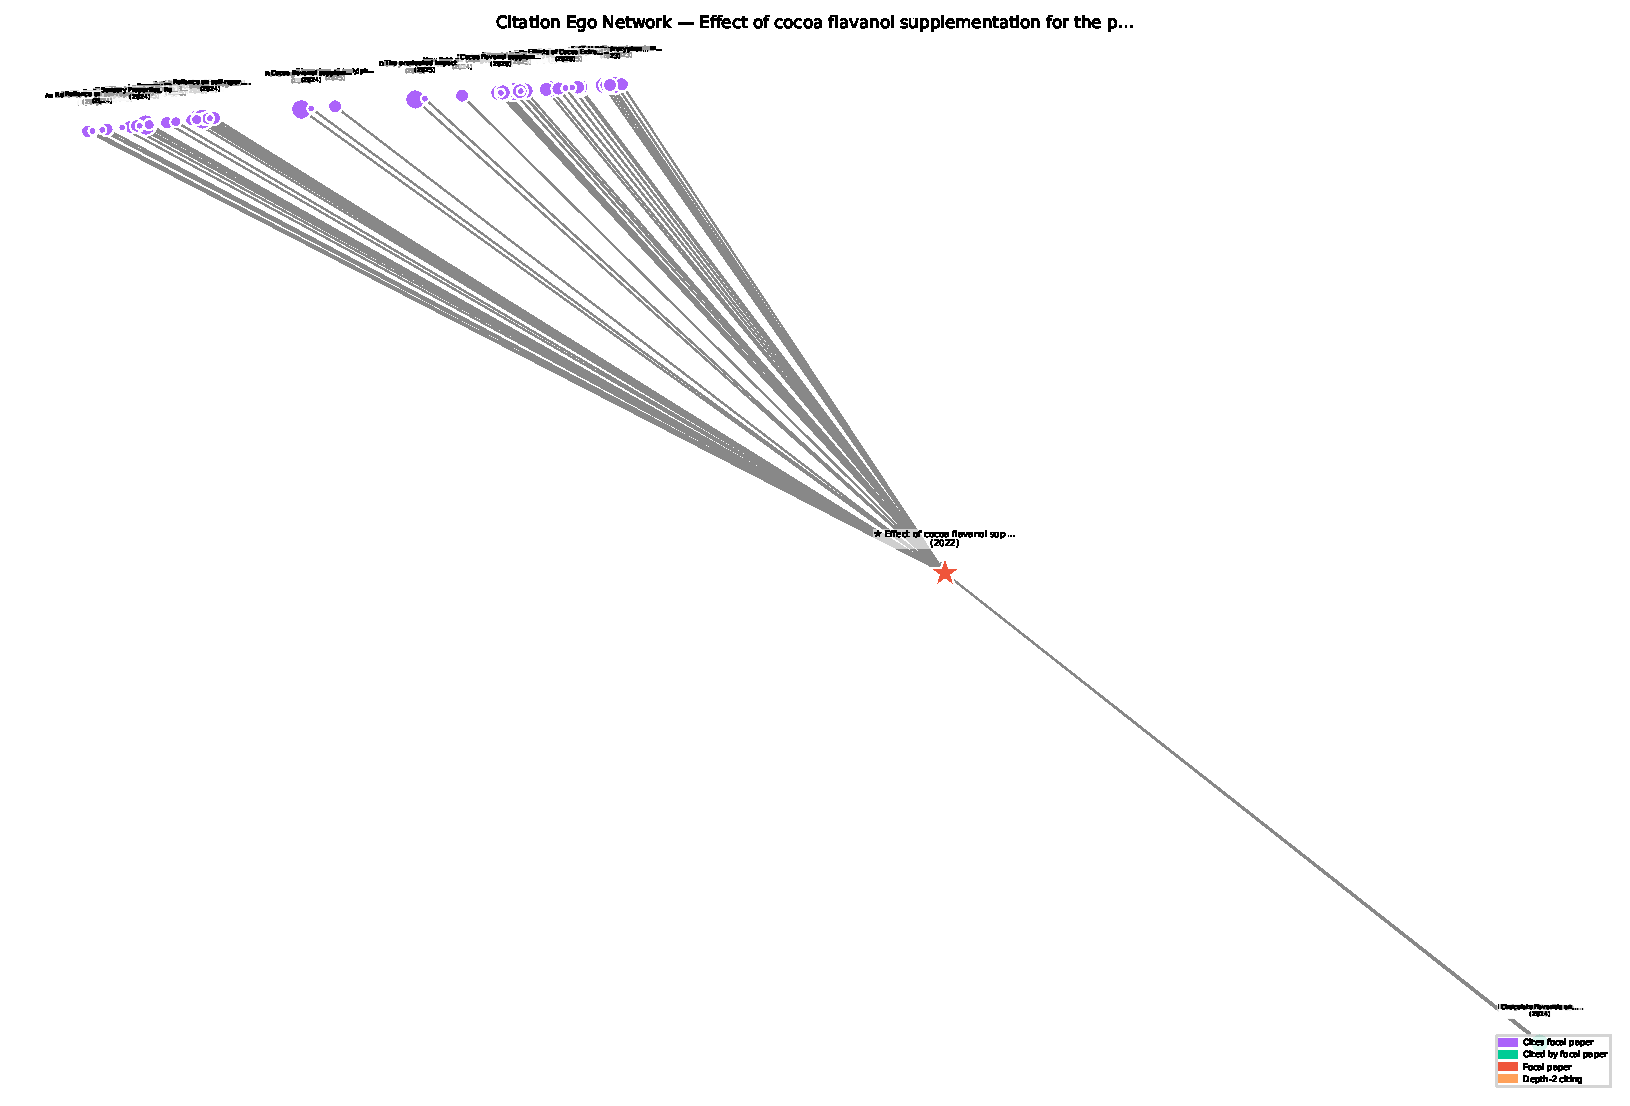
\includegraphics[width=\linewidth]{network_paper.pdf}

\noindent{\small
  \textcolor[RGB]{171,99,250}{Purple} = papers that cite this work;\;
  \textcolor[RGB]{0,204,150}{Green} = papers this work cites;\;
  \textcolor[RGB]{255,161,90}{Orange} = depth-2 citing papers.\;
  Node size $\propto$ $\log(\text{citations}+1)$.
  $\bigstar$ = focal paper.
}
\end{landscape}

\vfill
\noindent\rule{\linewidth}{0.4pt}\\
{\small Data source: \href{https://openalex.org}{OpenAlex}.
Network restricted to the Flavonoid research corpus.
Generated \today.}

\end{document}
